\documentclass[aspectratio=169]{beamer}

\graphicspath{{figures/}{../figures/}{../../paper/figures/}}

% Кириллица: pdfLaTeX -- через T2A, XeLaTeX/LuaLaTeX -- через системные шрифты.
\usepackage{iftex}
\ifPDFTeX
  \usepackage[T2A]{fontenc}
  \usepackage[utf8]{inputenc}
\else
  \usepackage{fontspec}
  \setsansfont{Arial}
\fi
\usepackage[english,russian]{babel}
\usepackage{amssymb,amsmath}
\usepackage{booktabs}
\usepackage{pgfplots}
\pgfplotsset{compat=1.17}

\usecolortheme{beaver}
\usefonttheme[onlymath]{serif}
\setbeamertemplate{navigation symbols}{}
\setbeamertemplate{footline}[frame number]
\setbeamersize{text margin left=0.5cm,text margin right=0.5cm}
\setbeamerfont{frametitle}{size=\normalsize}

% Цвета серий -- как на главном рисунке (code/plot.py).
\definecolor{cNone}{HTML}{BDBDBD}
\definecolor{cGsm}{HTML}{90CAF9}
\definecolor{cDapo}{HTML}{42A5F5}
\definecolor{cDeep}{HTML}{1565C0}
\definecolor{cCrisp}{HTML}{E67E22}

\title{CRISP: QA-датасет из сырых PDF\\с помощью самоигры Challenger--Reasoner}
\author{Роман Акрамов\\[2pt]\small Научный руководитель: Р.\,В.~Ищенко}
\date{Промежуточный доклад, 13.11.2026}

\begin{document}

% ---------- 1. Титул и цель ----------
\begin{frame}
\titlepage
\vspace{-14pt}
\centering\small
\textbf{Цель:} из PDF предметной области без ручной разметки получить QA-датасет\\
для SFT и RL, который обучает модель не хуже открытых датасетов.
\end{frame}

% ---------- 2. Однослайдовый ----------
\begin{frame}{Вопросы, сгенерированные из PDF без разметки, обучают модель на уровне открытых датасетов}
\vspace{-10pt}
\footnotesize
Qwen3-14B, один рецепт GRPO, меняются только обучающие данные. Метрика: acc@1 на 9 математических бенчмарках.
\centering
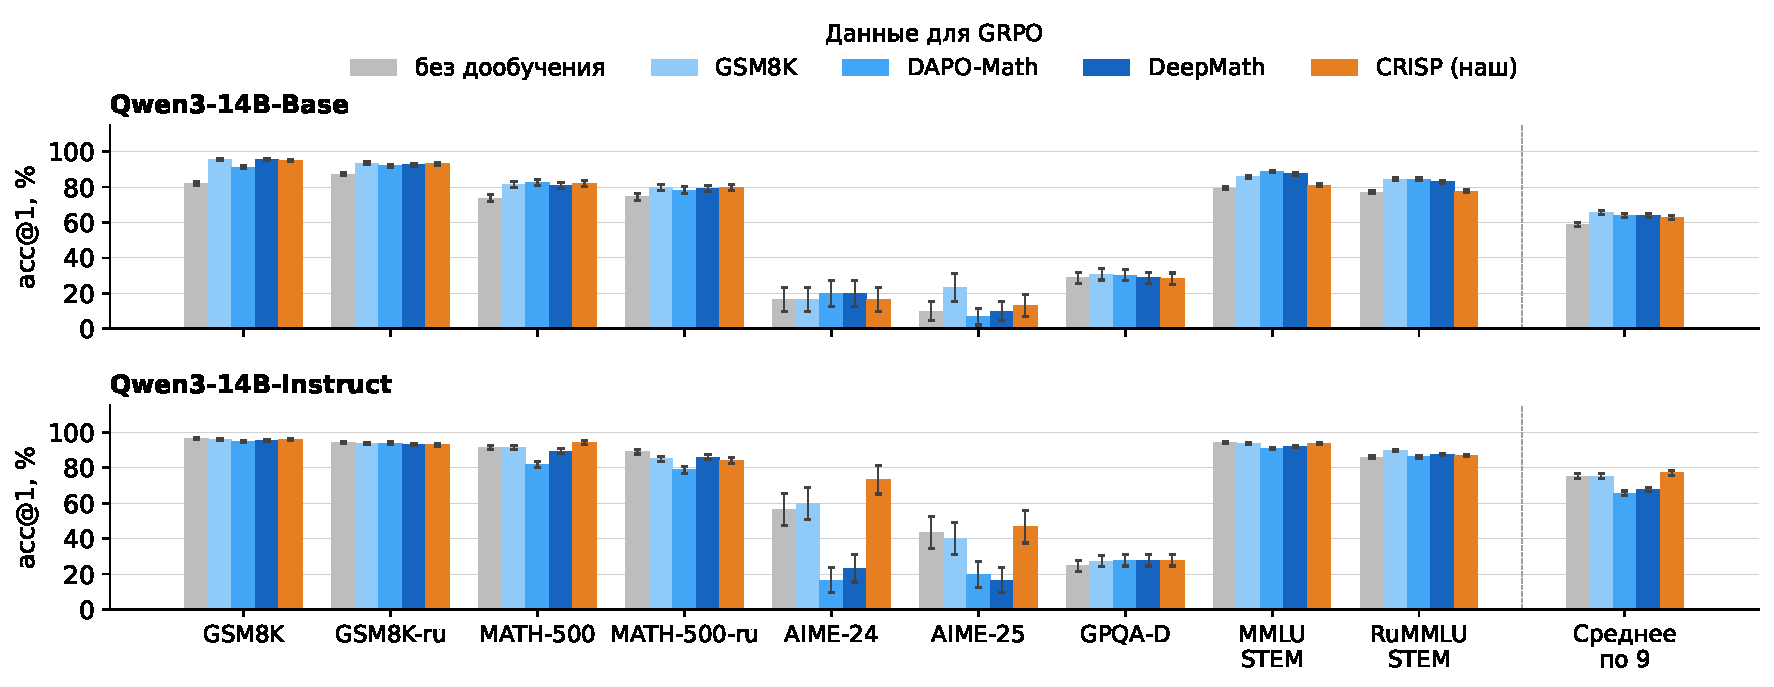
\includegraphics[width=0.9\textwidth]{oslide_main.pdf}

\raggedright
\textbf{Base:} прирост $+4.1$ п.п., у открытых датасетов от $+4.9$ до $+6.8$.
\quad \textbf{Instruct:} $+2.1$ п.п., DAPO-Math и DeepMath дают от $-7$ до $-10$.
\end{frame}

% ---------- 3. Литература ----------
\begin{frame}{RL-дообучению нужны вопросы с ответами, а существующие способы их получить не подходят узким областям}
\centering
\footnotesize
\begin{tabular}{lll}
\toprule
Работа & Что предлагает & Чего не хватает \\
\midrule
GRPO, Dr.\,GRPO (2024--2025) & RL с проверяемой наградой & нужны вопросы с ответами \\
Self-Instruct, WizardMath & дистилляция из учителя & ограничена знаниями учителя \\
R-Zero, Absolute Zero (2025) & самоигра без данных & галлюцинации, дрейф \\
SPICE (Liu et al., 2025) & самоигра по корпусу & код и данные закрыты, \\
& & на выходе модель, а не датасет \\
\midrule
\textbf{CRISP} & \textbf{самоигра по корпусу} & \textbf{открытый конвейер,} \\
& & \textbf{на выходе датасет} \\
\bottomrule
\end{tabular}

\vspace{8pt}
Награду за дисперсию и две роли берём из SPICE и встраиваем в конвейер от PDF до датасета.
\end{frame}

% ---------- 4. Постановка ----------
\begin{frame}{Постановка: датасет оценивается по приросту, который он даёт модели при фиксированном рецепте}
\small
\textbf{Модель.} Политика $\pi$ --- Qwen3-14B (Base или Instruct); $\mathrm{GRPO}(\pi, D)$ --- дообучение на датасете $D$ по одному рецепту.

\medskip
\textbf{Критерий.} Прирост точности относительно исходной модели:
\[
  \Delta(D) \;=\; \overline{\mathrm{acc@1}}\bigl(\mathrm{GRPO}(\pi, D)\bigr) \;-\; \overline{\mathrm{acc@1}}(\pi),
\]
где $\overline{\mathrm{acc@1}}$ --- среднее по 9 бенчмаркам, по 3 ответа на задачу при $T{=}0.6$.

\medskip
\textbf{Гипотеза.} Для датасета CRISP $D_C$, полученного без разметки, и открытых датасетов $D_{\text{open}}$ (GSM8K, DAPO-Math, DeepMath)
\[
  \Delta(D_C) \;\approx\; \Delta(D_{\text{open}}) \quad \text{в пределах шума оценки.}
\]
\end{frame}

% ---------- 5. Решение ----------
\begin{frame}{Решение: конвейер из четырёх этапов, вопросы рождаются в самоигре с наградой за дисперсию}
\begin{columns}[c]
\begin{column}{0.5\textwidth}
\centering
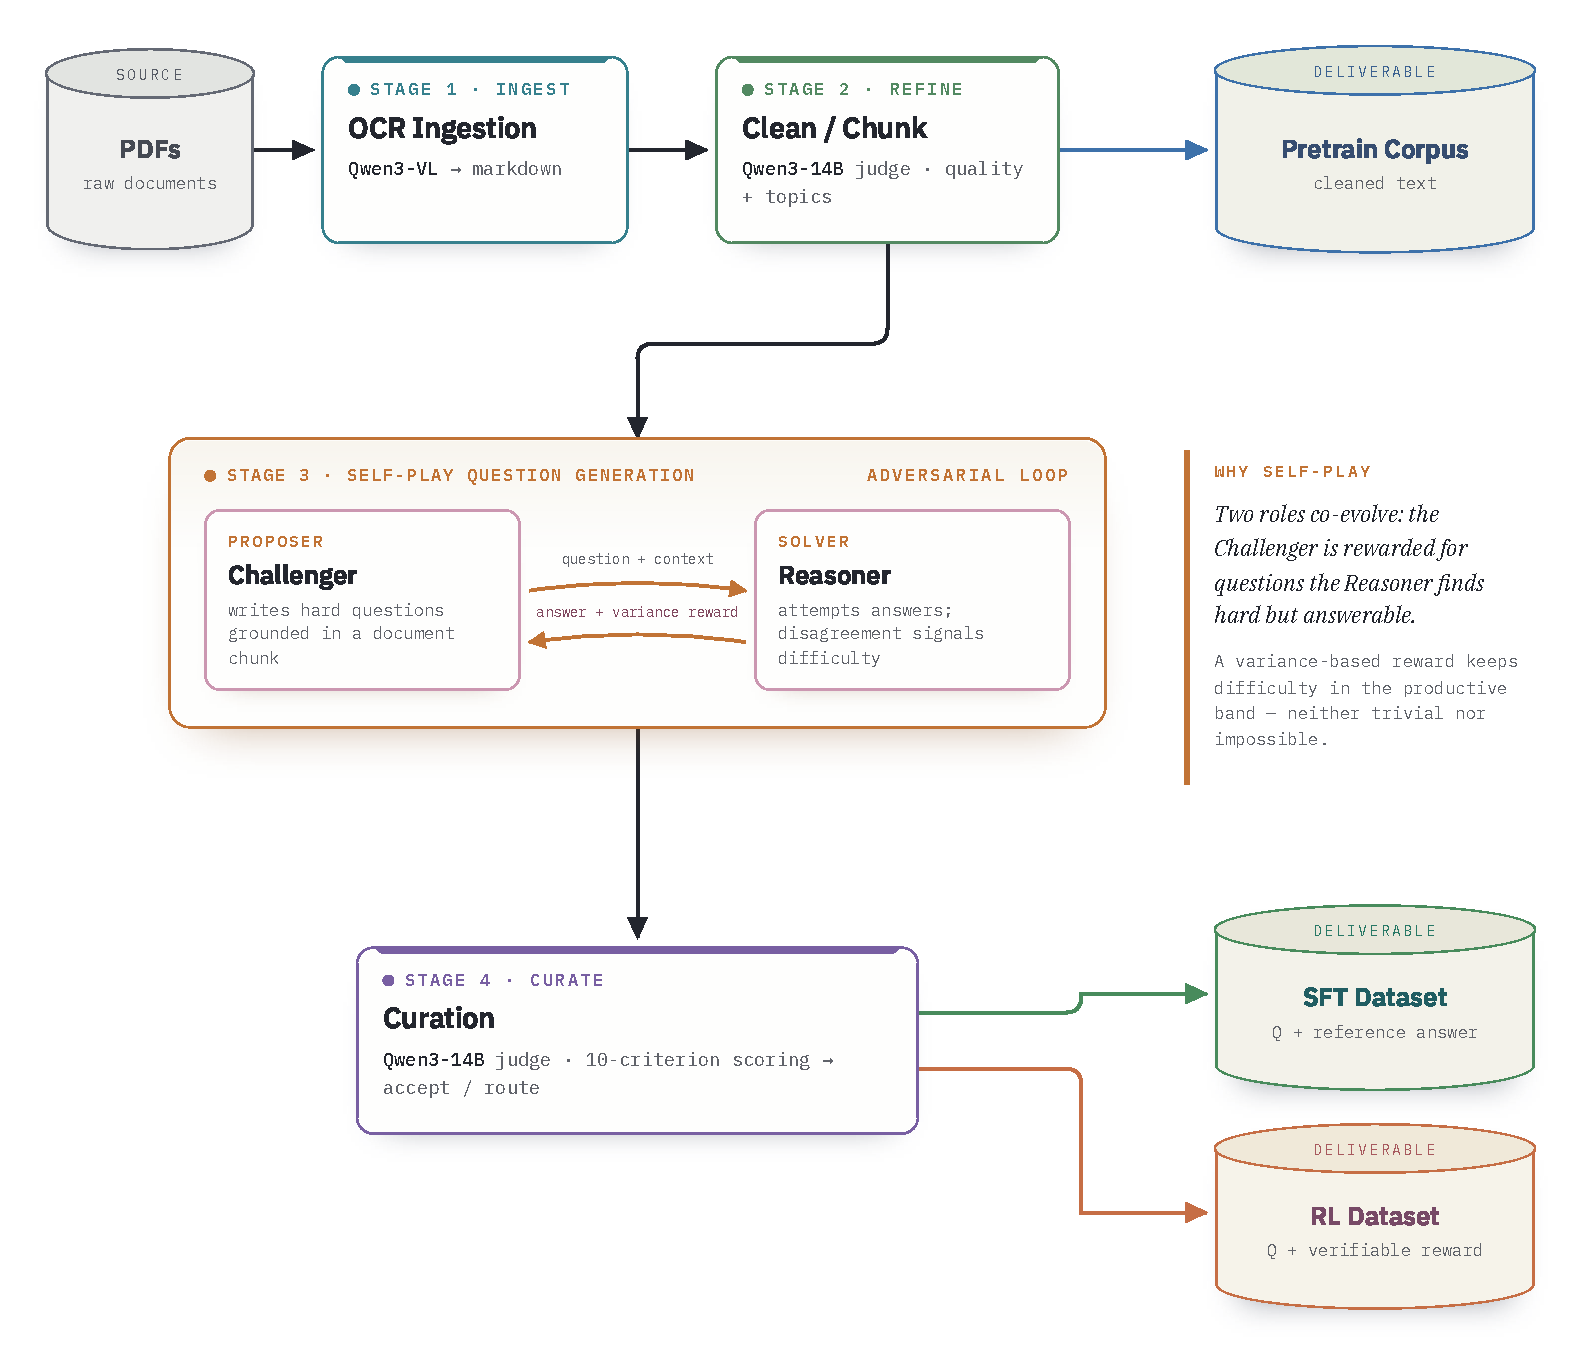
\includegraphics[height=0.72\textheight]{pipeline_factory.pdf}
\end{column}
\begin{column}{0.48\textwidth}
\small
\textbf{Challenger} видит фрагмент документа и задаёт вопрос, \textbf{Reasoner} отвечает без документа $K$ раз; $\bar\ell$ --- доля верных ответов.
\[
  r_C = \exp\!\Bigl(-\frac{(v - 0.25)^2}{2 \cdot 0.01}\Bigr),
  \quad v = \bar\ell\,(1-\bar\ell)
\]
\centering
\begin{tikzpicture}
\begin{axis}[
  width=0.95\linewidth, height=0.36\textheight,
  xlabel={$\bar\ell$}, ylabel={$r_C$},
  xmin=0, xmax=1, ymin=0, ymax=1.05,
  xtick={0,0.5,1}, ytick={0,1},
  label style={font=\scriptsize},
  tick label style={font=\scriptsize},
]
\addplot[domain=0:1, samples=200, thick, color=red!60!black]
  {exp(-((x*(1-x)) - 0.25)^2 / (2*0.01))};
\end{axis}
\end{tikzpicture}

\raggedright
Слишком лёгкие и нерешаемые вопросы награды не получают.
\end{column}
\end{columns}
\end{frame}

% ---------- 6. Эксперимент и анализ ошибки ----------
\begin{frame}{Эксперимент: на Base CRISP отстаёт от DAPO-Math и DeepMath меньше, чем шум оценки}
\small
\textbf{Цели:} сравнить CRISP с тремя открытыми датасетами при одном рецепте GRPO; проверить на слабой (Base) и сильной (Instruct) модели.
\textbf{Ошибка:} усы --- $\pm1$ std биномиального шума среднего по 9 бенчмаркам.

\centering
\begin{tikzpicture}
\begin{axis}[
  ybar, bar width=9pt,
  width=0.9\textwidth, height=0.5\textheight,
  ymin=55, ymax=80,
  ylabel={среднее acc@1, \%},
  symbolic x coords={Base,Instruct},
  xtick=data, enlarge x limits=0.5,
  legend style={font=\scriptsize, at={(0.5,1.02)}, anchor=south, legend columns=5, draw=none},
  label style={font=\scriptsize},
  tick label style={font=\scriptsize},
  error bars/y dir=both, error bars/y explicit,
]
\addplot[fill=cNone, draw=none] coordinates {(Base,58.9) +- (0,1.10) (Instruct,75.2) +- (0,1.48)};
\addplot[fill=cGsm, draw=none] coordinates {(Base,65.7) +- (0,1.24) (Instruct,75.2) +- (0,1.47)};
\addplot[fill=cDapo, draw=none] coordinates {(Base,63.8) +- (0,1.07) (Instruct,65.7) +- (0,1.21)};
\addplot[fill=cDeep, draw=none] coordinates {(Base,64.1) +- (0,1.12) (Instruct,67.9) +- (0,1.23)};
\addplot[fill=cCrisp, draw=none] coordinates {(Base,63.0) +- (0,1.13) (Instruct,77.3) +- (0,1.42)};
\legend{без дообучения, GSM8K, DAPO-Math, DeepMath, CRISP}
\end{axis}
\end{tikzpicture}

\raggedright
Шум среднего $\approx 1$--$1.5$ п.п., на отдельном AIME (30 задач) --- до 9 п.п.: выводы делаем по среднему. GSM8K на Base выше CRISP на 2.7 п.п. --- это больше шума.
\end{frame}

% ---------- 7. Итог ----------
\begin{frame}{Итог: вопросы из PDF без разметки дают прирост на уровне открытых датасетов}
\centering
\small
\begin{tabular}{lcccc}
\toprule
& \multicolumn{2}{c}{Qwen3-14B-Base} & \multicolumn{2}{c}{Qwen3-14B-Instruct} \\
\cmidrule(lr){2-3}\cmidrule(lr){4-5}
Данные GRPO & acc@1, \% & $\Delta$, п.п. & acc@1, \% & $\Delta$, п.п. \\
\midrule
без дообучения & $58.9 \pm 1.1$ & --- & $75.2 \pm 1.5$ & --- \\
GSM8K & $65.7 \pm 1.2$ & $+6.9$ & $75.2 \pm 1.5$ & $+0.1$ \\
DAPO-Math & $63.8 \pm 1.1$ & $+4.9$ & $65.7 \pm 1.2$ & $-9.5$ \\
DeepMath & $64.1 \pm 1.1$ & $+5.3$ & $67.9 \pm 1.2$ & $-7.2$ \\
\textbf{CRISP (наш)} & $\mathbf{63.0 \pm 1.1}$ & $\mathbf{+4.1}$ & $\mathbf{77.3 \pm 1.4}$ & $\mathbf{+2.1}$ \\
\bottomrule
\end{tabular}

\vspace{8pt}
\raggedright
\textbf{Выводы.} На Base прирост того же порядка (на уровне DAPO-Math и DeepMath, ниже GSM8K), на Instruct CRISP не ухудшает модель ($+2.1$), а DAPO-Math и DeepMath снижают точность на 7--10 п.п.
\end{frame}

\end{document}
